\chapter{Analyse et spécifications des besoins}

{\LARGE \bfseries Introduction\\[0.4cm] }
\\ Ce chapitre a pour objectif de définir et d’analyser les besoins du système Persona Tester afin de garantir une conception cohérente et adaptée aux attentes des utilisateurs. Il présente d’abord les spécifications fonctionnelles et non fonctionnelles, ainsi que les différents acteurs du système. Cette étape permet de traduire les objectifs du projet en exigences techniques claires. Elle constitue une base essentielle pour les phases de conception et de réalisation.\\

Les besoins définis dans ce chapitre constituent la base de la stratégie de validation du système. Chaque exigence fonctionnelle sera vérifiée à travers des tests adaptés : les tests unitaires valideront les composants isolés tels que le générateur de personas et le compresseur de snapshots, les tests d'intégration vérifieront les interactions entre l'agent, le serveur MCP et le LLM, et les tests système valideront l'ensemble du pipeline de bout en bout.



\section{Spécifications des besoins}
Cette section a pour objectif de présenter les spécifications des besoins du système Persona Tester. Elle regroupe l’identification des acteurs ainsi que la définition des besoins fonctionnels et non fonctionnels. Elle permet de formaliser les exigences essentielles du système avant sa conception.

\subsection{Identification des acteurs }  
Les acteurs du système représentent l’ensemble des entités, qu’elles soient humaines ou logicielles, qui interagissent avec la plateforme afin d’exécuter différentes tâches et assurer son bon fonctionnement. Chaque acteur possède un rôle spécifique et des responsabilités bien définies au sein du système Persona Tester.\\



\subsubsection{Acteurs primaires}

\begin{itemize}

\item \textbf{Utilisateur / Testeur UX} : acteur principal du système, il configure les paramètres de test, soumet les URLs, valide les personas générés et lance les simulations. Il analyse également les résultats .\\

\item \textbf{Système de génération} : ensemble de composants basés sur des modèles de langage permettant d’analyser un site web, de générer des personas comportementaux et de produire des scénarios de navigation exploitables.\\

\item \textbf{Agent d’exécution (PersonaAgent)} : composant autonome simulant un utilisateur réel dans un navigateur. Il prend des décisions dynamiques via une boucle ReAct et interagit avec le site en temps réel.\\

\end{itemize}

\subsubsection{Acteurs secondaires}

\begin{itemize}

\item \textbf{Serveur MCP Playwright} : couche d’abstraction permettant d’exécuter des actions navigateur (clic, navigation, saisie) et de retourner les états de page.\\

\item \textbf{Serveur MCP custom} : serveur complémentaire fournissant des outils avancés comme l’extraction du DOM nettoyé et l’exécution de scripts Playwright autonomes.\\

\item \textbf{Modèle de langage (LLM)} : moteur intelligent assurant plusieurs rôles : analyse de site, génération de personas, planification de scénarios et prise de décision dynamique.\\

\item \textbf{Base de données} : système de persistance stockant les sites analysés, les personas, les scénarios, ainsi que les traces d’exécution.\\

\end{itemize}

%--------------------------------------------------

\subsection{Besoins fonctionnels}

Les besoins fonctionnels décrivent les fonctionnalités que le système doit offrir afin de répondre aux attentes de ses différents acteurs. Ils sont organisés par acteur afin de garantir une traçabilité claire entre les fonctionnalités et les responsabilités dans le pipeline.\\

\subsubsection{Besoins liés à l'utilisateur}

\begin{itemize}
\item Soumettre une URL et un objectif de test via le dashboard.\\
\item Configurer le nombre de personas et les contraintes démographiques.\\
\item Consulter et modifier les personas générés.\\
\item Réviser et ajuster les scénarios avant exécution.\\
\item Lancer l’exécution d’un persona sur un site cible.\\
\item Visualiser les résultats, traces d’exécution et screenshots.\\
\item Accéder à l’historique des tests et aux statistiques.\\
\end{itemize}

\subsubsection{Besoins liés au système de génération}

\begin{itemize}
\item Analyser automatiquement un site web via un crawl navigateur.\\
\item Extraire les fonctionnalités, formulaires et flux utilisateurs.\\
\item Générer un contexte LLM structuré.\\
\item Produire plusieurs personas cohérents partageant un objectif commun.\\
\item Générer des scénarios composés d’actions ordonnées.\\
\item Persister les données générées en base de données.\\
\end{itemize}

\subsubsection{Besoins liés à l’agent d’exécution}

\begin{itemize}
\item Charger les personas et scénarios depuis la base de données.\\
\item Construire un comportement basé sur les caractéristiques du persona.\\
\item Exécuter une boucle ReAct (observer, raisonner, agir).\\
\item Interagir dynamiquement avec le site web.\\
\item Gérer les éléments bloquants (popups, modales).\\
\item Enregistrer chaque étape d’exécution.\\
\item Retourner un statut final (succès, échec, abandon).\\
\end{itemize}

\subsubsection{Besoins liés au serveur MCP custom}

\begin{itemize}
\item Fournir un DOM nettoyé exploitable par le LLM.\\
\item Exécuter des scripts Playwright en mode autonome.\\
\item Retourner les logs d’exécution et les screenshots.\\
\item Gérer le cycle de vie du navigateur.\\
\end{itemize}

\subsubsection{Besoins liés à la base de données}

\begin{itemize}
\item Stocker les sites analysés et leurs métadonnées.\\
\item Persister les personas et leurs profils comportementaux.\\
\item Enregistrer les scénarios et les plans d’action.\\
\item Conserver les traces d’exécution détaillées.\\
\item Fournir des données pour les statistiques du dashboard.\\
\end{itemize}

%--------------------------------------------------

\subsection{Besoins non fonctionnels}

Les besoins non fonctionnels définissent les contraintes de qualité et les exigences techniques du système. Ils garantissent sa robustesse, sa performance et sa maintenabilité.\\

\begin{itemize}

\item \textbf{Robustesse} : le système doit être capable de gérer les erreurs, les échecs d’appel au LLM et les situations imprévues via des mécanismes de retry et de gestion des exceptions.\\

\item \textbf{Performance} : les données transmises au modèle doivent être optimisées afin de respecter les contraintes de taille et de temps de réponse, notamment via la compression des pages web.\\

\item \textbf{Isolation des sessions} : chaque exécution doit être indépendante afin d’éviter toute contamination entre les tests (cookies, cache, sessions).\\

\item \textbf{Traçabilité} : toutes les actions effectuées par l’agent doivent être enregistrées afin de permettre une analyse détaillée des exécutions.\\

\item \textbf{Extensibilité} : l’architecture doit permettre l’ajout de nouveaux outils et serveurs MCP sans modifier le cœur du système.\\

\item \textbf{Interopérabilité LLM} : le système doit fonctionner avec différents fournisseurs de modèles de langage sans modification majeure.\\

\item \textbf{Maintenabilité} : le code doit être structuré de manière modulaire avec une séparation claire entre frontend et backend.\\

\end{itemize}

\subsection{Analyse des besoins}

Cette section a pour objectif de décrire et de formaliser les besoins identifiés pour la plateforme \textit{Persona Tester}. Elle met en évidence les interactions entre les différents acteurs et le système à travers des diagrammes de cas d’utilisation, ainsi que les principaux flux du pipeline de génération et d’exécution. Ces représentations permettent de mieux comprendre le fonctionnement global du système et constituent une base essentielle pour les phases de conception et de développement.\\

\subsubsection{Diagramme de cas d’utilisation}

Le diagramme de cas d’utilisation illustre les interactions entre les différents acteurs du système \textit{Persona Tester} et les fonctionnalités qu’il propose. Il permet d’identifier les rôles de chaque acteur ainsi que leurs interactions avec le pipeline de génération de personas et d’exécution des tests.

La figure 2.1 présente une vue globale des interactions entre les acteurs identifiés et les principales fonctionnalités du système.








\begin{figure}[H]
\begin{center}
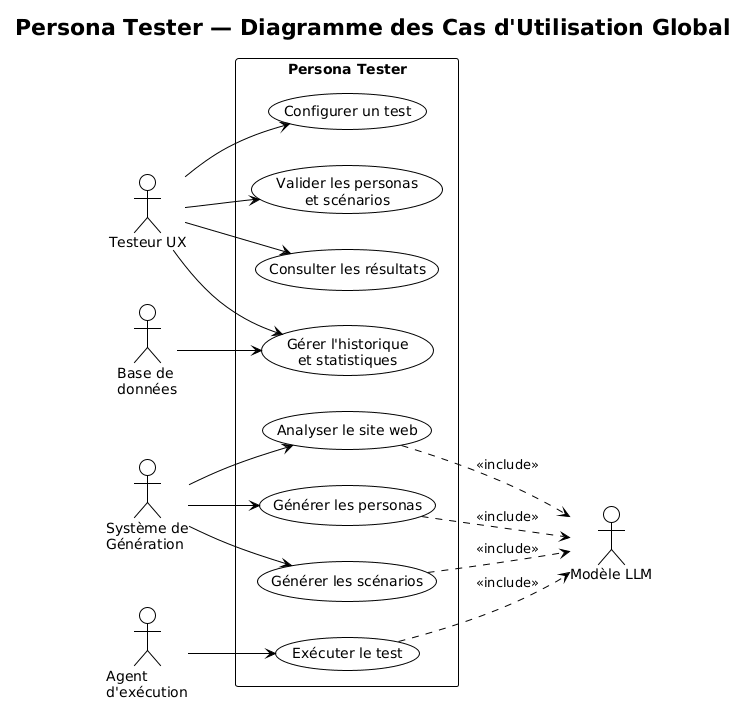
\includegraphics[height=150mm]{images/diagramme-usecase.png}
\end{center}
\caption{Diagramme de cas d’utilisation du système }
\end{figure}
\section{Conception}
\subsubsection{Architecture physique}

L’architecture physique du projet \textit{Persona Automation} repose sur une séparation claire des responsabilités entre trois couches principales. Cette organisation favorise l’évolutivité du système, notamment pour l’intégration ou le changement de modèles d’intelligence artificielle, tout en améliorant sa modularité et sa maintenabilité.\\

\begin{itemize}

\item \textbf{Niveau Présentation (Presentation Tier)} : il correspond à l’interface utilisateur développée en React et TypeScript. C’est la couche avec laquelle l’utilisateur interagit afin de configurer les tests, consulter les résultats, éditer les scénarios générés et visualiser l’historique des exécutions.\\

\item \textbf{Niveau Application (Application Tier)} : il constitue le cœur du système. Il regroupe le backend développé avec FastAPI, responsable de la coordination des flux, ainsi que la couche d’intelligence artificielle composée d’agents tels que \textit{WebsiteAnalyzer} et \textit{PersonaGenerator}, basés sur des modèles comme Ollama ou OpenAI. Cette couche inclut également le moteur d’exécution Playwright, chargé de simuler les interactions utilisateur dans le navigateur.\\

\item \textbf{Niveau Données (Data Tier)} : il repose sur une base de données SQLite assurant la persistance des données. Ce niveau stocke l’ensemble des artefacts générés par le système, notamment les profils de personas, les scénarios de navigation, les captures d’écran ainsi que les logs détaillés des exécutions.\\

\end{itemize}

\begin{figure}[H]
\begin{center}
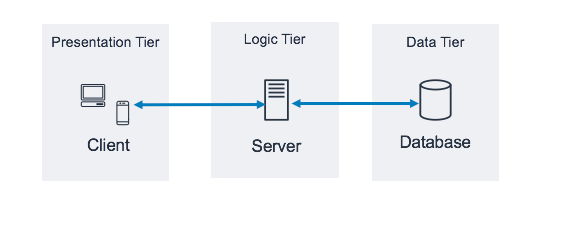
\includegraphics[height=70mm]{images/Architecture-physique-tiers.png}
\end{center}
\caption{Architecture physique 3-tiers }
\end{figure}

%-------------------------------------------------------

\subsubsection{Architecture logique}

L’architecture logique adoptée pour ce système suit également une structure en trois tiers, décrivant l’organisation fonctionnelle des composants logiciels et facilitant la maintenance ainsi que l’auditabilité des tests.\\

\begin{itemize}

\item \textbf{Couche de présentation} : elle gère les interactions avec l’utilisateur à travers l’interface React. Des composants tels que \textit{App.tsx} assurent l’orchestration des tâches, tandis que \textit{ScriptModal.tsx} permet une validation humaine (human-in-the-loop) avant l’exécution des scénarios.\\

\item \textbf{Couche applicative (métier)} : elle représente le cœur fonctionnel du système. Elle transforme l’analyse d’un site web en intentions de navigation via un pipeline structuré : Analyse → Génération de Personas → Planification d’actions. Cette couche intègre également un agent autonome basé sur le pattern ReAct (Observation → Raisonnement → Action), permettant une adaptation dynamique à l’état réel du site web.\\

\item \textbf{Couche de données} : elle assure la persistance et la traçabilité de toutes les informations du système. Contrairement à un simple outil de test, elle conserve chaque étape intermédiaire du processus, incluant les analyses JSON, les métadonnées des personas et les logs d’exécution, permettant ainsi une analyse comparative et une amélioration continue du système.\\


\begin{figure}[H]
\begin{center}
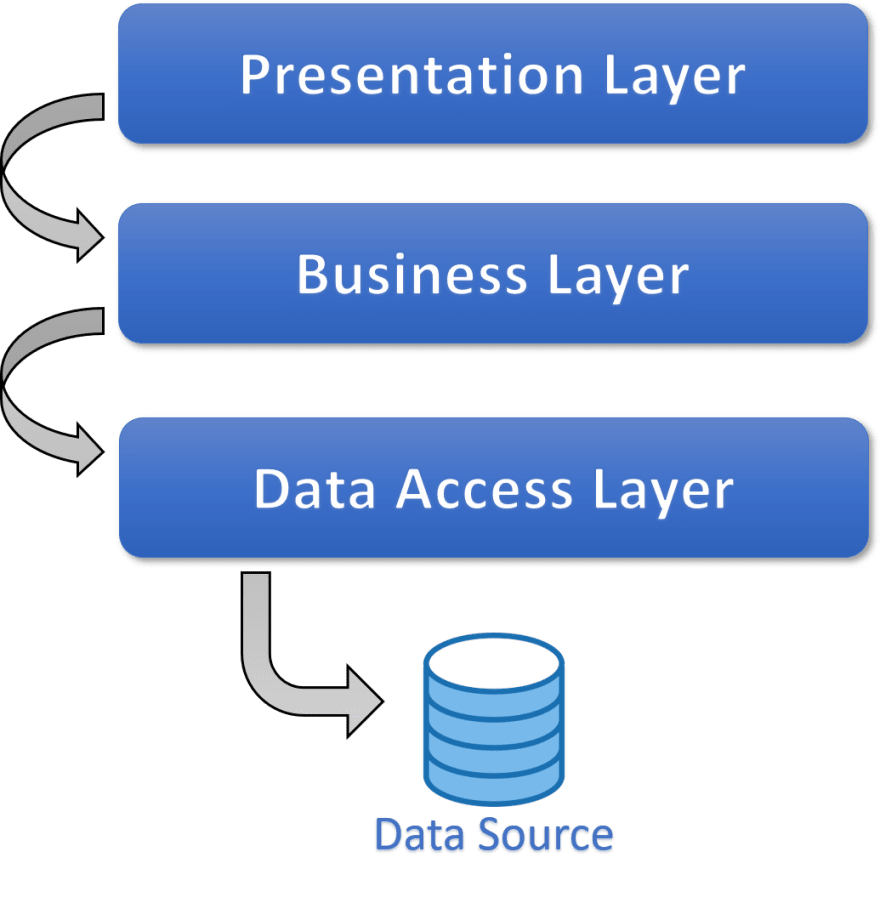
\includegraphics[height=70mm]{images/Architecture-logique.png}
\end{center}
\caption{Architecture logique 3-tiers }
\end{figure}

\end{itemize}

\subsection{Planification du projet avec Scrum}

Dans le cadre du développement du projet \textit{Persona Tester}, la méthodologie Agile Scrum a été adoptée afin d’assurer une gestion itérative et flexible du projet. Cette approche permet de découper le développement en plusieurs sprints, facilitant ainsi l’adaptation aux évolutions des besoins et l’amélioration continue du système.\\

Le travail est organisé sous forme de backlog produit, regroupant l’ensemble des fonctionnalités à développer sous forme de \textit{user stories}. Chaque élément du backlog est priorisé et estimé afin de planifier efficacement les sprints et suivre l’avancement global du projet.\\

%--------------------------------------------------

\subsection{Backlog Produit}

Le backlog produit regroupe l’ensemble des user stories du projet, organisées par épic et classées selon leur priorité. Chaque fonctionnalité est estimée en points de complexité (Story Points) et associée à un état d’avancement, permettant de suivre l’évolution du projet.\\






\renewcommand{\arraystretch}{1.4}

\begin{center}
\small
\begin{longtable}{|c|p{3.5cm}|c|p{7cm}|}
\hline
\rowcolor{gray!20}
\textbf{ID-F} & \textbf{Features} & \textbf{ID-Us} & \textbf{User Stories} \\
\hline
\endfirsthead

\hline
\rowcolor{gray!20}
\textbf{ID-F} & \textbf{Features} & \textbf{ID-Us} & \textbf{User Stories} \\
\hline
\endhead

% ================= EP-01 =================
\multirow{6}{*}{1} & 
\multirow{6}{3.5cm}{Analyse de site web} 
& 1.1 & En tant que système, je veux crawler un site avec plusieurs stratégies progressives afin de maximiser le taux de succès. \\ \cline{3-4}

& & 1.2 & En tant que système, je veux extraire les fonctionnalités clés, formulaires et flux utilisateurs. \\ \cline{3-4}

& & 1.3 & En tant que système, je veux enrichir l'analyse via recherche web en cas d'échec du scraping. \\ \cline{3-4}

& & 1.4 & En tant qu'utilisateur, je veux soumettre une URL et un objectif de test via le dashboard. \\ \cline{3-4}

& & 1.5 & En tant qu'utilisateur, je veux sauvegarder les analyses en base de données. \\ \cline{3-4}

& & 1.6 & En tant qu'utilisateur, je veux désactiver le scraping si nécessaire. \\

\hline

% ================= EP-02 =================
\multirow{6}{*}{2} & 
\multirow{6}{3.5cm}{Génération de personas} 

& 2.1 & En tant que système, je veux générer plusieurs personas réalistes partageant un objectif commun. \\ \cline{3-4}

& & 2.2 & En tant que système, je veux adapter les personas aux contraintes démographiques configurées. \\ \cline{3-4}

& & 2.3 & En tant que système, je veux valider les attributs des personas générés. \\ \cline{3-4}

& & 2.4 & En tant que système, je veux persister les personas en base de données. \\ \cline{3-4}

& & 2.5 & En tant qu'utilisateur, je veux consulter et modifier les personas générés avant exécution. \\ \cline{3-4}

& & 2.6 & En tant qu'utilisateur, je veux configurer le nombre de personas et leurs contraintes démographiques. \\

\hline

% ================= EP-03 =================
\multirow{5}{*}{3} & 
\multirow{5}{3.5cm}{Génération de scénarios} 

& 3.1 & En tant que système, je veux générer des scénarios composés d'actions ordonnées adaptées au profil du persona. \\ \cline{3-4}

& & 3.2 & En tant que système, je veux valider la cohérence du scénario par rapport au persona associé. \\ \cline{3-4}

& & 3.3 & En tant que système, je veux sauvegarder les scénarios en base de données. \\ \cline{3-4}

& & 3.4 & En tant qu'utilisateur, je veux visualiser et modifier les scénarios avant exécution. \\ \cline{3-4}

& & 3.5 & En tant qu'utilisateur, je veux valider manuellement un scénario avant de lancer le test. \\

\hline

% ================= EP-04 =================
\multirow{6}{*}{4} & 
\multirow{6}{3.5cm}{Exécution de l'agent} 

& 4.1 & En tant que système, je veux exécuter une boucle ReAct pour simuler le comportement d'un utilisateur réel. \\ \cline{3-4}

& & 4.2 & En tant que système, je veux optimiser les données transmises au LLM afin de respecter les contraintes de taille. \\ \cline{3-4}

& & 4.3 & En tant que système, je veux gérer les erreurs et les retry LLM de manière automatique. \\ \cline{3-4}

& & 4.4 & En tant que système, je veux enregistrer chaque étape d'exécution avec captures d'écran. \\ \cline{3-4}

& & 4.5 & En tant que système, je veux limiter la durée d'exécution d'un agent pour éviter les boucles infinies. \\ \cline{3-4}

& & 4.6 & En tant que système, je veux gérer les éléments bloquants (popups, modales) de manière autonome. \\

\hline

% ================= EP-05 =================
\multirow{4}{*}{5} & 
\multirow{4}{3.5cm}{Persistance \& Traçabilité} 

& 5.1 & En tant que système, je veux stocker les sites analysés et leurs métadonnées en base de données. \\ \cline{3-4}

& & 5.2 & En tant que système, je veux conserver les traces d'exécution détaillées pour chaque session de test. \\ \cline{3-4}

& & 5.3 & En tant que système, je veux assurer l'isolation des sessions pour éviter toute contamination entre les tests. \\ \cline{3-4}

& & 5.4 & En tant qu'utilisateur, je veux accéder à l'historique complet des tests effectués. \\

\hline

% ================= EP-06 =================
\multirow{6}{*}{6} & 
\multirow{6}{3.5cm}{Interface \& Visualisation} 


& 6.1 & En tant qu'utilisateur, je veux un dashboard affichant les statistiques globales des tests. \\ \cline{3-4}

& & 6.2 & En tant qu'utilisateur, je veux une interface de configuration des paramètres de test. \\ \cline{3-4}

& & 6.3 & En tant qu'utilisateur, je veux lancer un test complet en un seul clic. \\ \cline{3-4}

& & 6.4 & En tant qu'utilisateur, je veux visualiser les logs et screenshots en temps réel. \\ \cline{3-4}

& & 6.5 & En tant qu'utilisateur, je veux comparer les résultats entre plusieurs personas sur le même site. \\ \cline{3-4}

& & 6.6 & En tant qu'utilisateur, je veux générer et exécuter des scripts Playwright depuis l'interface. \\

\hline

\end{longtable}
\end{center}

\subsubsection{Planification des sprints}

Pour assurer une bonne organisation du développement de la plateforme 
\textit{Persona Tester}, le projet a été découpé en quatre sprints 
successifs, reflétant l'évolution réelle du projet depuis la prise en 
main de Playwright jusqu'à l'observabilité complète du système.

\begin{itemize}

% ===================== SPRINT 1 =====================
\item \textbf{Sprint 1 : Prise en main de Playwright et premier 
pipeline d'exécution MCP}

L'objectif de ce sprint est de valider la faisabilité technique de 
l'automatisation navigateur et d'intégrer le protocole MCP pour 
piloter Playwright via un agent LLM. Les principales tâches 
réalisées sont :

\begin{itemize}
    \item Prise en main de Playwright : écriture et exécution de 
    scripts de navigation classiques sur des sites cibles.
    \item Validation de la faisabilité : interactions avec formulaires, 
    clics, captures d'écran et navigation multi-pages.
    \item Intégration du serveur MCP Playwright : connexion stdio, 
    exposition des outils navigateur à l'agent.
    \item Implémentation de la boucle ReAct (\textit{Observation → 
    Raisonnement → Action}) pour piloter la navigation.
    \item Création de scénarios de test décrits en langage naturel 
    et exécutés via MCP.
    \item Mise en place de l'environnement backend : FastAPI, SQLite, 
    structure du projet Python.
    \item Développement du dashboard React initial : soumission d'URL, 
    visualisation des logs et screenshots.
    \item Premiers tests d'exécution sur des sites cibles 
    (\textit{automationexercise.com}, \textit{demoblaze.com}).
\end{itemize}

\textbf{Livrable :} Pipeline MCP fonctionnel, boucle ReAct opérationnelle, 
dashboard initial livré, premiers scénarios exécutés avec succès.

% ===================== SPRINT 2 =====================
\item \textbf{Sprint 2 : Génération de personas et simulation 
comportementale}

Ce sprint constitue le cœur fonctionnel du projet. Il est dédié à 
l'implémentation du moteur de génération de personas et à la validation 
de la divergence comportementale entre profils. Les tâches principales 
sont :

\begin{itemize}
    \item Implémentation d'une première version de génération de 
    personas : profils variés avec objectifs différents pour explorer 
    les fonctionnalités d'un site web donné.
    \item Optimisation du pipeline : génération de plusieurs personas 
    partageant un \textbf{même objectif} mais avec des \textbf{comportements 
    différents} (impatient, méthodique, novice, expert, etc.).
    \item Intégration du formulaire de configuration dans le dashboard : 
    nombre de personas, contraintes démographiques, objectif de test.
    \item Exécution des personas générés sur des sites cibles et 
    observation de la divergence comportementale.
    \item Persistance des personas et de leurs profils comportementaux 
    en base de données SQLite.
    \item Mise en place de la factory LLM multi-fournisseurs (Groq, 
    GitHub Models, Google Gemini, Ollama).
\end{itemize}

\textbf{Livrable :} Pipeline de génération de personas fonctionnel, 
divergence comportementale prouvée entre personas, données persistées 
en base.

% ===================== SPRINT 3 =====================
\item \textbf{Sprint 3 : Optimisation du crawl et gestion de 
l'authentification}

Ce sprint est dédié à l'amélioration de la qualité du contexte transmis 
au LLM pour la génération des personas, ainsi qu'à la gestion des sites 
nécessitant une authentification. Il inclut :

\begin{itemize}
    \item Intégration de \textit{crawl4ai} pour le crawl intelligent 
    du site cible : extraction structurée du contenu, rendu JavaScript, 
    conversion HTML vers Markdown.
    \item Enrichissement du contexte LLM : fourniture d'une description 
    précise des fonctionnalités, formulaires et flux du site pour 
    améliorer la qualité des personas générés.
    \item Gestion des sites débutant par une page de login : intégration 
    de Playwright (et Browser-Use pour les interfaces complexes) pour 
    effectuer l'authentification avant le crawl.
    \item Développement du serveur MCP custom : extraction du DOM 
    nettoyé, exécution de scripts Playwright autonomes.
    \item Optimisation de la compression des snapshots DOM pour 
    respecter les contraintes de taille du contexte LLM.
    \item Tests de régression sur les sites déjà validés pour vérifier 
    la non-régression après optimisation.
\end{itemize}

\textbf{Livrable :} Crawl intelligent opérationnel, gestion du login 
intégrée, qualité de génération des personas améliorée et mesurée.

% ===================== SPRINT 4 =====================
\item \textbf{Sprint 4 : Observabilité avec OpenTelemetry et 
validation finale}

Ce dernier sprint vise à instrumenter la plateforme avec OpenTelemetry 
afin de collecter des données d'observabilité complètes sur l'ensemble 
du pipeline, et à valider le système de bout en bout. Il comprend :

\begin{itemize}
    \item Intégration d'OpenTelemetry dans le backend FastAPI et 
    le moteur d'exécution de l'agent.
    \item Collecte des \textbf{traces} : suivi du parcours complet 
    d'une session de test, de la soumission de l'URL jusqu'au 
    résultat final.
    \item Collecte des \textbf{logs} : enregistrement structuré des 
    événements d'exécution, erreurs LLM et actions navigateur.
    \item Collecte des \textbf{métriques} : mesure des performances 
    (temps de génération, taux de succès, nombre de retry LLM, 
    durée d'exécution par persona).
    \item Visualisation des données d'observabilité dans le dashboard.
    \item Tests end-to-end de l'ensemble du pipeline instrumenté et 
    validation finale de la plateforme.
\end{itemize}

\textbf{Livrable :} Plateforme complète instrumentée avec OpenTelemetry, 
métriques et traces disponibles dans le dashboard, validation 
end-to-end réalisée.

\end{itemize}

\subsection{Environnement de travail}


Dans cette section, nous présentons l’environnement matériel et logiciel utilisé pour le développement, les tests et l’exécution de la plateforme \textit{Persona Tester}.\\


\subsubsection{Environnement matériel}

Le tableau 2.2 présente la configuration matérielle de la machine principale utilisée pour le développement du projet.

\begin{table}[H]
\centering
\begin{tabular}{|c|c|}
\hline
\textbf{Composant} & \textbf{Spécification} \\
\hline
Processeur & Intel Core i7-13650HX (13ème génération, 2.60 GHz) \\
\hline
Mémoire RAM & 14 Go \\
\hline
Stockage & 475 Go SSD \\
\hline
Carte graphique & NVIDIA GeForce RTX 4050 \\
\hline
\end{tabular}
\caption{Environnement matériel utilisé}
\end{table}

\subsubsection{Environnement logiciel}

L’environnement logiciel du projet \textit{Persona Tester} regroupe l’ensemble des technologies utilisées pour le développement, l’orchestration des agents IA, l’automatisation des navigateurs ainsi que la mise en place du frontend et du backend. Afin de faciliter la compréhension, ces technologies sont organisées en plusieurs catégories.

\paragraph{Langages de programmation}

Le projet repose principalement sur les langages suivants :
\begin{itemize}
    \item Python : utilisé pour le développement du backend, des agents IA et du moteur d’orchestration.
    \item TypeScript : utilisé pour le développement du frontend afin d’assurer la robustesse du code.
    \item JavaScript : utilisé indirectement via l’écosystème React et Node.js.
\end{itemize}

\paragraph{Frameworks et bibliothèques}

Le projet s’appuie sur plusieurs frameworks et bibliothèques essentielles :

\begin{itemize}
    \item FastAPI : framework backend principal pour la création des API REST.
    \item React 19 : bibliothèque frontend pour la construction de l’interface utilisateur.
    \item Vite : outil de build et serveur de développement frontend.
    \item LangChain  : orchestration des agents IA et des workflows LLM.
    \item Playwright : automatisation des interactions navigateur.
    \item MCP (Model Context Protocol) : interface d’exécution des actions navigateur.
    \item Crawl4AI : extraction et analyse de contenu web.
    \item requests : gestion des requêtes HTTP.
\end{itemize}

\paragraph{Environnement de développement}

Le développement du projet a été réalisé dans les environnements suivants :

\begin{itemize}
    \item Python 3.10+ pour l’exécution du backend.
    \item Node.js 18+ pour le frontend React.
    \item VS Code comme environnement principal de développement.
    \item Git et GitHub pour le contrôle de version et la collaboration.
\end{itemize}

\paragraph{Outils et infrastructure}

Les outils et services suivants ont été utilisés pour l’exécution et l’intégration du système :

\begin{itemize}
    \item Ollama : exécution locale des modèles de langage (LLM).
    \item Modèle par défaut : \textit{qwen3.5:cloud}.
    \item OpenAI API : fallback cloud pour les modèles IA.
    \item Google Gemini API : alternative pour les LLM.
    \item GitHub Models : support de modèles supplémentaires.
    \item SQLite : base de données légère pour la persistance locale.
    \item Playwright Chromium : navigateur automatisé pour les tests.
\end{itemize}

\paragraph{Variables d’environnement}

Les principales variables utilisées dans le projet sont :
\begin{itemize}
    \item \texttt{OLLAMA\_BASE\_URL}
    \item \texttt{OLLAMA\_MODEL}
    \item \texttt{OPENAI\_API\_KEY}
    \item \texttt{GOOGLE\_API\_KEY}
    \item \texttt{GITHUB\_TOKEN}
\end{itemize}

\section{Conclusion}

Ce chapitre a permis de définir les besoins fonctionnels et non fonctionnels du système \textit{Persona Tester}, ainsi que d’identifier les différents acteurs et leurs interactions avec la plateforme. Il a également présenté la planification du projet selon la méthodologie Scrum, ainsi que l’environnement matériel et logiciel utilisé pour le développement. Ces éléments constituent une base essentielle pour la phase de conception détaillée du système.